\section{The agent's own options: paying a debt}
\label{sec:own}

\subsection{Quitting and continuing across all 188 debts}
A debt gives the agent a local goal with a known endpoint: raise a stated amount or leave the game. The one decision that needs foresight is whether to continue. Once an agent continues, the menu refreshes after each action and shows what can be done next. An agent that quits has judged the whole route from the first menu.

Table~\ref{tab:debt} and Figure~\ref{fig:debt}A partition the \fact{d.episodes} episodes by what payment required at the first menu. In \fact{d.above-bound.episodes} the debt exceeded everything the player owned. The agent declared bankruptcy at the first menu in \fact{d.above-bound.declared-at-first-menu} of them and sold or mortgaged first in \fact{x.debt.above.continued}. In the \fact{d.payable} payable debts the agent continued in \fact{x.debt.payable.continued} and quit at the first menu in \fact{x.debt.payable.declared}. Agents paid \fact{d.classes.paid} of the \fact{d.payable}, with \fact{d.paid-actions.mortgages} mortgages and \fact{d.paid-actions.sales} building sales and no engine fallback. The remaining elimination, Opus in G7, had assets above the debt on paper, but its menu offered no building sale. The bank had no houses left, so its one hotel could not be broken down, and that blocked the rest of the group.

\begin{table}[t]\centering\small
\TableDebt
\caption{All \fact{d.episodes} debt episodes. Rows one to three split the \fact{d.payable} payable debts by the least the first menu required. ``Quit at first menu'' counts bankruptcy declared as the first action. The \fact{x.debt.above.continued} other debts above every asset ended in elimination after some liquidation.}
\label{tab:debt}\end{table}

Most payable debts were easy. In \fact{d.tiers-among-payable.listed.episodes} of them, cash and the mortgages already on the menu covered the debt, and \fact{d.paid-actions.single-action} of the \fact{d.classes.paid} payments took one action. The median paid debt was \fact{x.debt.median.ratio.pct}\% of the debtor's asset bound. The overall payment rate of \fact{x.debt.payable.paid.pct}\% therefore says little about difficulty. The table does show discrimination at the first menu. The agents quit almost always when no payment existed and almost never when one did. This is level three: the choice agrees with the arithmetic of the state.

\begin{figure}[t]\centering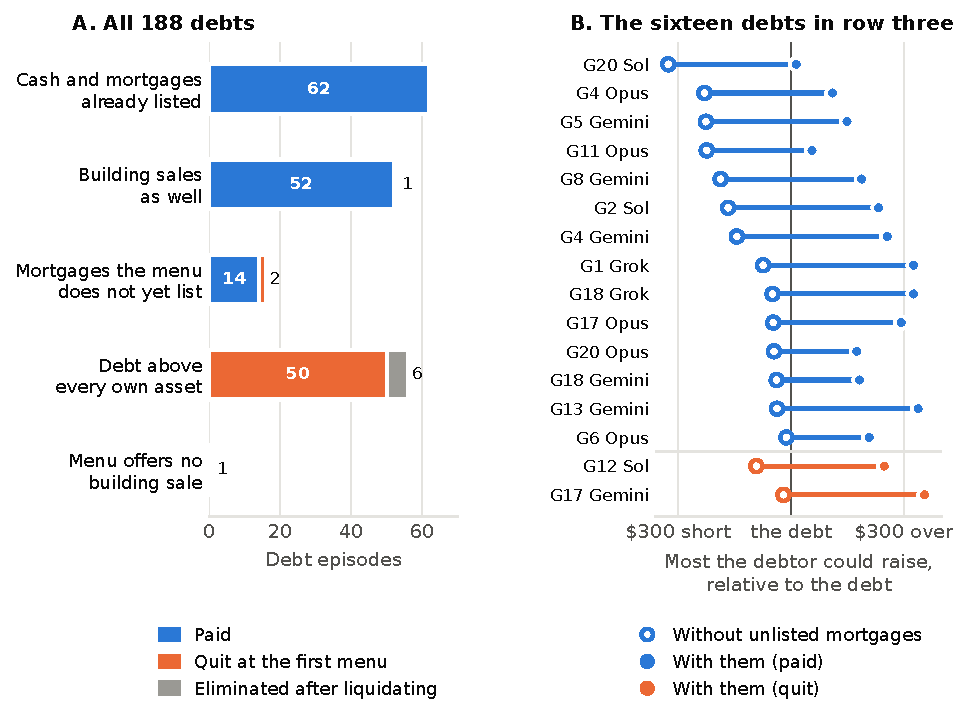
\includegraphics[width=\linewidth]{debt_partition.pdf}
\caption{Debts and what they required. A: every debt episode, by the least the first menu required and by outcome. B: the sixteen debts in the third row. The open circle is the most the debtor could raise from cash, listed mortgages and all building sales. The filled circle adds the mortgages that selling those buildings would release. Every case starts short of the debt and ends beyond it. The two debtors that quit are at the bottom.}
\label{fig:debt}\end{figure}

\subsection{Sixteen debts that needed mortgages the menu did not list}
The third row of Table~\ref{tab:debt} is the hard set. In these sixteen episodes, cash plus every listed mortgage plus the sale of every building still fell short, by a median of \$\fact{d.necessary.median-shortfall-without-unlisted} (Figure~\ref{fig:debt}B). Payment had to use deeds that the first menu did not offer and that no prompt mentions as a resource. An agent that adds up what the menu lists concludes that it cannot pay.

Agents paid fourteen of the sixteen (Table~\ref{tab:sixteen}). Thirteen began by selling buildings, one mortgaged a listed deed first, and all fourteen then mortgaged at least one released deed. The payments took two to ten actions, with a median of \fact{d.necessary.median-actions-paid}. The cases come from twelve games and all five seed blocks, and every system has at least two.

\begin{table}[t]\centering\footnotesize
\TableSixteen
\caption{The sixteen payable debts that required unlisted mortgages. ``Reach without unlisted'' is cash plus listed mortgages plus full building salvage. ``Channel'' is where the text stored at the first decision comes from: the applied private note, or the provider-returned explanation where Opus answered through action-only recovery. The next column is the drafting assistant's reading of what that text does with the unlisted mortgages, with exact spans in Appendix~\ref{app:debts}.}
\label{tab:sixteen}\end{table}

The text stored at the first decision separates the outcomes. In thirteen of the fourteen payments it counts the unlisted mortgages before any building is sold. Gemini's note in G5 is typical:
\TranscriptQuote{g5-d263-note}
The provider-returned text of the same response shows the sum being revised: \InlineQuote{in-g5-d263-revise} The fourteenth payment, Opus in G20, raises the released mortgages as a question without a total. In both failures the text adds up the listed items only. Gemini in G17 held the same two dark-blue deeds it had counted in G5:
\TranscriptQuote{g17-d234-note}
Park Place and Boardwalk would have added \$375 after the sales. Sol in G12 left out \$340 of red mortgages in the same way:
\TranscriptQuote{g12-d190-note}
Both agents declared bankruptcy in that response. Sol counts released mortgages in G2 and in G20.

Nine of the fourteen successful texts are applied private notes, which the same agent reads on later turns. Five are Opus's provider-returned explanations, because recovery responses carry no note. The stated figures can be checked. Of \fact{x.nc.numbers.checked} stated totals, gaps or remainders, \fact{x.nc.numbers.equal} equal the value computed from the records. The exception is Sol's \$430 for yellow mortgages worth \$400, which did not affect the payment. Since the prompt supplies none of these values, each one is a board fact the system recalled.

This result reaches level three with accurate content. The statement comes before the action, its arithmetic is correct in all but one case, and the choice to continue or quit agrees with it in all sixteen. It does not reach level four. No pair of cases differs only in the unlisted collateral, and two failures cannot show that the omission produced the bankruptcy. The text also does not show how the choice was computed.

\subsection{One payment followed from both sides}
\IncidentTitle{g20pay}{A creditor's estimate and a debtor's plan agree on \$1,414}
At G20 turn 107 only Gemini and Sol remain. Sol has \$49, nine orange houses and two brown hotels. Before adding a hotel that raises one rent to \$1,400, Gemini writes down what Sol could raise:
\TranscriptQuote{g20-d325-creditor}
Sol lands there on the next turn. Its first menu lists three mortgageable deeds worth \$325, and its note states a budget before any action:
\TranscriptQuote{g20-d327-plan}
Sol sells its development in two actions and mortgages eight deeds, five of them released by the sales. Its note at the last one reads:
\TranscriptQuote{g20-d336-last}
The events show \$700 from sales and \$665 from mortgages, so $49+700+665-1{,}400=14$. Gemini's total was also right, although its two components were each off by \$25 in opposite directions. Sol was eliminated seven turns later and Gemini won.
\IncidentSource{G20 d325 and d327 to d336, standard responses. All three quotations are private notes and were not delivered to the other player. Sales, mortgages, the rent and the \$14 balance are read from events and the next prompt.}

The case shows an announced total carried through ten applied actions to the dollar. Sol stated one aggregate budget and a rule, to sell everything and then mortgage everything. Once the buildings were gone, the eight mortgages could be made in any order, and each refreshed menu showed what remained. Ten actions are not ten steps of lookahead. What Sol fixed in advance was the total, the decision not to concede, and the reliance on \$340 of collateral that the first menu did not list.

Nineteen payments used a mortgage that was absent from the first menu. Fourteen are the cases above. In the other five the released deeds were one way to pay among several. The third payable bankruptcy, Grok in G12, was not a failed sum. Its note says \InlineQuote{in-g12-d249-note} The text outside its tool call names a two-house sale, and the call that arrived declared bankruptcy.
